
\chapter{Methodology}

In order to evaluate the different control algorithms and their performance, the approach towards designing and testing the algorithms must be systematic and concise. 
The different subproblems specified in \ref{intro:sub_problems}, can be said to either relate to either the simulation design or the algorithm design. As such, for the purpose of this thesis, a different approach will be used when dealing with constructing the simulation and when designing and testing the control algorithms. In this chapter, I will outline these approaches and the methodology used. 

\section{Control Problem}
The main research problem os this thesis involves building and evaluating different control algorithms, and as such each algorithm must be subject to the same evaluation technique.
This evaluation technique will throughout the thesis be referenced to as the \textit{Control Problem}, and the purpose of the agents will be so solve this problem collectively. 
As such the problem chosen must be the same problem throughout every simulation and independent of the control algorithms themselves. The problem must also be able to be solved collectively, by multiple agents at the same time, while still posing enough challenges to properly test the control algorithms. Posing dangers to the agents, such as the risk of collision. 

This control problem will exist within the simulation as a physical task that the agents have to carry out. Chapter \ref{}


\section{Simulation construction}

\section{Validation}

\section{Metrics}

\section{Experimentation}

\section{Optimization}



\begin{figure}[h!]
  \centering
  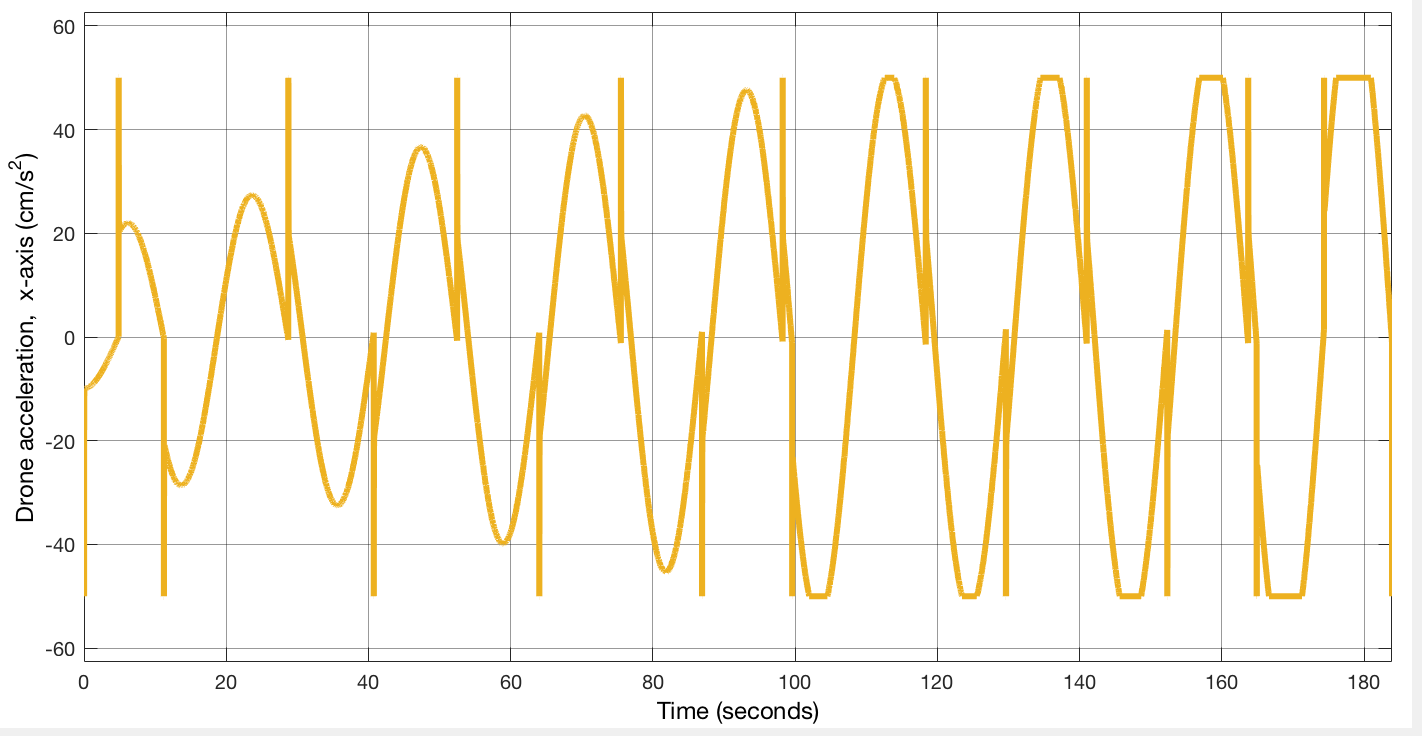
\includegraphics[width=.8\columnwidth]{figures/SA_accel_with_no_vel_limit.png}
  \caption{Acceleration of agent - without velocity limit}
  \label{fig:sa_accel_no_vel_adj}
\end{figure}






